%-----------------------------------------------------------------------------%
\chapter{\babTiga}
%-----------------------------------------------------------------------------%
Penelitian ini bertujuan untuk mengevaluasi konfigurasi Hypervisor KVM yang disediakan secara default dalam konteks penggunaan \vm\ pada Apache Cloudstack. Tujuan utama adalah untuk memastikan bahwa \vm\ dapat mencapai kinerja yang optimal sesuai dengan spesifikasi sistem yang digunakan. Untuk mencapai tujuan ini, \saya\ akan melakukan penyesuaian konfigurasi atau konfigurasi pada Hypervisor KVM dan kemudian membandingkannya dengan kondisi awal yang tidak mengalami konfigurasi. Hasil pengujian akan dianalisis untuk menentukan apakah ada perbedaan signifikan dalam kinerja antara Hypervisor KVM yang telah dikonfigurasikan dengan yang belum dikonfigurasikan.

%-----------------------------------------------------------------------------%
\section{Tahapan Penelitian}
%-----------------------------------------------------------------------------%
\begin{figure}
    \centering
    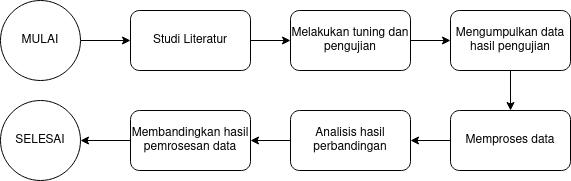
\includegraphics[width=1\textwidth]
    {assets/pics/tahapan-penelitian.png}
    \caption{Tahapan Penelitian}
    \label{fig:TahapanPenelitian}
\end{figure}

Penelitian ini akan dilakukan dalam beberapa tahap sesuai dengan diagram di gambar \ref{fig:TahapanPenelitian}. Tahap pertama melibatkan studi literatur untuk mengumpulkan semua informasi yang diperlukan. Studi literatur ini penting karena memberikan dasar pengetahuan yang kuat tentang topik yang akan diteliti, memungkinkan peneliti untuk memahami konteks dan kerangka kerja yang relevan.

Selanjutnya, penelitian melibatkan konfigurasi terhadap Hypervisor KVM, dan pengujian dilakukan dengan tiga skenario, yaitu kompresi video, enkripsi dan dekripsi dengan AES, dan validasi integritas data menggunakan CRC32. Hasil dari pengujian ini akan memberikan gambaran mengenai konfigurasi yang paling optimal dan sesuai, serta membantu dalam pemahaman lebih lanjut tentang pengaruh konfigurasi terhadap performa Hypervisor KVM.

%-----------------------------------------------------------------------------%
\section{Persiapan Lingkungan untuk Pengujian dan Analisis}
%-----------------------------------------------------------------------------%
\begin{figure}
    \centering
    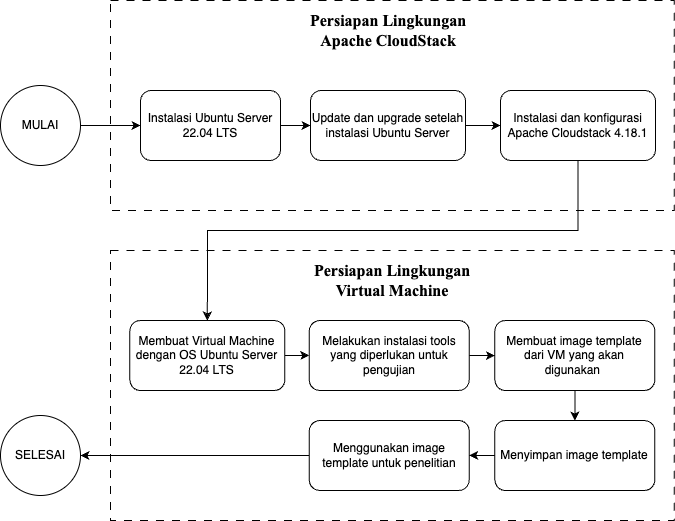
\includegraphics[width=1\textwidth]
    {assets/pics/persiapan_lingkungan_penelitian.png}
    \caption{Persiapan Lingkungan Penelitian}
    \label{fig:PersiapanLingkunganPenelitian}
\end{figure}


Proses persiapan lingkungan untuk pengujian dan analisis yang tergambar dalam gambar \ref{fig:PersiapanLingkunganPenelitian} menggambarkan serangkaian langkah sistematis yang penting untuk memastikan integritas hasil penelitian. Proses ini dimulai dengan tahap inisiasi yang meliputi instalasi Ubuntu Server 22.04 LTS, sebuah sistem operasi yang stabil dan sering digunakan untuk keperluan server. Instalasi ini menjadi landasan dasar bagi infrastruktur yang akan dikembangkan.

Setelah sistem operasi terinstal, dilakukan pembaruan dan peningkatan sistem operasi tersebut untuk memastikan semua komponen sistem berada pada versi terkini serta keamanan sistem terjaga. Langkah ini krusial untuk menutup potensi kerentanan yang mungkin ada pada sistem. Selanjutnya, Apache Cloudstack versi 4.18.1 diinstal dan dikonfigurasikan. Apache Cloudstack berfungsi sebagai platform manajemen cloud yang memungkinkan pembuatan dan pengelolaan infrastruktur cloud yang kompleks, yang merupakan elemen kunci dalam penelitian ini.

Dalam pembuatan lingkungan virtual, dibuat \vm\ yang menggunakan sistem operasi yang sama, yaitu Ubuntu Server 22.04 LTS. Pembuatan VM ini memungkinkan simulasi berbagai skenario penelitian dalam lingkungan yang terisolasi. Selanjutnya, untuk keperluan analisis dan pengujian, berbagai perangkat lunak yang akan digunakan untuk melakukan pengujian akan di install.

Tahapan selanjutnya merupakan pembuatan image template dari VM yang telah dikonfigurasikan. Proses ini memungkinkan duplikasi VM dengan cepat dan efisien untuk pengujian berulang atau skenario analisis yang berbeda, menjamin konsistensi lingkungan penelitian. Image template ini kemudian digunakan sebagai standar untuk penelitian lebih lanjut, memastikan bahwa setiap VM yang dibuat untuk tujuan pengujian memiliki konfigurasi yang identik.

Setelah semua dilakukan hal ini menandakan bahwa lingkungan penelitian telah siap untuk diuji dan dianalisis. Kesiapan lingkungan ini esensial untuk memastikan bahwa pengujian yang dilakukan dapat diulang dengan cepat dan efisien.


%-----------------------------------------------------------------------------%
\subsection{Konfigurasi Apache CloudStack}
%-----------------------------------------------------------------------------%

\begin{figure}
    \centering
    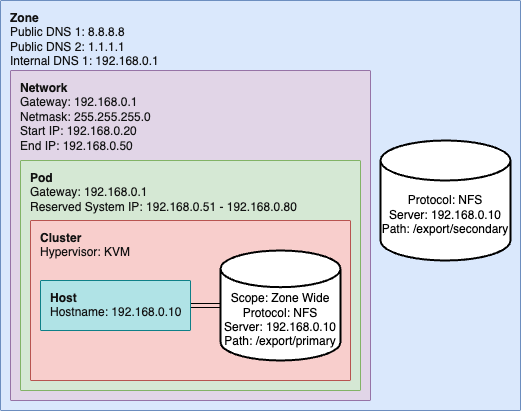
\includegraphics[width=1\textwidth]
    {assets/pics/cloudstack_config.png}
    \caption{Konfigurasi Apache CloudStack}
    \label{fig:KonfigurasiApacheCloudStack}
\end{figure}

Pada gambar \ref{fig:KonfigurasiApacheCloudStack}, terlihat konfigurasi Apache CloudStack yang \saya\ terapkan. Pada Zone, \saya\ menggunakan public DNS yaitu \texttt{8.8.8.8} dan \texttt{1.1.1.1}, yang merupakan DNS publik dari Google dan Cloudflare. Sementara untuk DNS internal, \saya\ menggunakan IP \texttt{192.168.0.1} yang merupakan IP gateway di jaringan Home Network. Untuk Network, \saya\ menetapkan IP \texttt{192.168.0.1} sebagai gateway untuk mengarahkan seluruh traffic dari CloudStack ke jaringan \f{Home Network} \saya. Netmask yang \saya\ gunakan adalah \texttt{255.255.255.0}, dimana memiliki total IP yang dapat dipakai hingga 254 IP dalam jaringan \f{Home Network} untuk CloudStack.

Rentang IP di Network \saya\ tetapkan dari \texttt{192.168.0.20} hingga \texttt{192.168.0.50}, yang artinya terdapat 30 IP yang tersedia untuk VM yang akan dibuat. Pada Pod, \saya\ menggunakan IP \texttt{192.168.0.1} sebagai gateway dan \f{Reserved System IP} dari \texttt{192.168.0.51} hingga \texttt{192.168.0.80}. \f{Reserved System IP} ini merupakan sistem yang dibuat oleh CloudStack secara otomatis yang menjalankan fungsi seperti manajemen jaringan, \f{load balancing}, dan lain-lain. Pada Cluster, \saya\ menggunakan KVM sebagai Hypervisor dengan Host IP di \texttt{192.168.0.10}, yang merupakan IP dari host yang akan digunakan oleh CloudStack.

Untuk Primary Storage, \saya\ menggunakan protokol NFS dengan cakupan Zone Wide pada server \texttt{192.168.0.10} dan path \texttt{/export/primary}, yang mana Primary Storage adalah penyimpanan yang nanti akan digunakan untuk operasi \vm\ secara langsung. Sedangkan untuk Secondary Storage, \saya\ menggunakan protokol NFS pada server \texttt{192.168.90.10} dengan path \texttt{/export/secondary}, yang mana Secondary Storage adalah penyimpanan yang digunakan untuk menyimpan data yang jarang diakses secara langsung oleh \vm\ ataupun sistem dari CloudStack.

%-----------------------------------------------------------------------------%
\subsection{Persiapan \vm}
%-----------------------------------------------------------------------------%
Pada tahap ini akan dijelaskan bagaimana cara \saya\ membuat \vm\ yang akan digunakan untuk melakukan pengujian. \vm\ yang akan dibuat menggunakan image Ubuntu Server 22.04 LTS yang telah diinstal sebelumnya.

%-----------------------------------------------------------------------------%
\subsubsection{Image Ubuntu Server 22.04 LTS}
%-----------------------------------------------------------------------------%
Langkah pertama yang \saya\ lakukan adalah mengunduh file image ISO Ubuntu Server 22.04 LTS dari situs resmi Ubuntu dan menyimpannya di sistem host. Agar dapat digunakan oleh CloudStack, file ISO ini perlu di-hosting agar dapat diakses melalui alamat IP host. Hosting ini akan dilakukan menggunakan Apache2, sebuah aplikasi web server. Setelah konfigurasi Apache2 selesai dan file image ISO dapat diakses melalui alamat IP, selanjutnya \saya\ membuka CloudStack dan menuju ke \texttt{Configuration>Global Settings>All Settings}. Di sini, \saya\ akan mengisi konfigurasi \texttt{"Secstorage allow internal sites"} dengan nilai \texttt{192.168.0.0/24} (Home network) dan menyimpan pengaturan tersebut. Setelah itu, \saya\ pergi ke \texttt{Images>ISOs} dan memilih opsi "register ISO". Kemudian \saya\ menambahkan file ISO Ubuntu Server 22.04 LTS yang telah diunduh sebelumnya dengan memasukkan alamat URL image ISO dari sistem host.

%-----------------------------------------------------------------------------%
\subsubsection{Membuat Image Template}
%-----------------------------------------------------------------------------%
Setelah ISO image sudah siap digunakan langkah selanjutnya yang \saya\ lakukan adalah membuat image template dengan pergi ke \texttt{Compute>Instances} dan memilih "Add Instances". Konfigurasi \vm\ yang digunakan \saya\ adalah seperti ini:

\begin{enumerate}
    \item Deployment Infrastructure
          \begin{itemize}
              \item Pod: Default
              \item Cluster: Default
              \item Host: Default
          \end{itemize}

    \item Template/ISO

          ISO Ubuntu Server 22.04 LTS

    \item Compute Offering

          \saya\ memilih tipe High Instance dengan spesifikasi:
          \begin{itemize}
              \item CPU: 4 vCPU
              \item Clock Speed: 2.0 GHz
              \item Memory: 4096 MB
          \end{itemize}

    \item Data Disk

          Pada penelitian ini \vm\ akan diberikan data disk berukuran 20GB.

    \item Networks

          Di bagian jaringan, \saya\ membuat jaringan baru untuk digunakan oleh \vm\ dengan menggunakan template \texttt{"Network Offering used for CloudStack Kubernetes Service"} dan mengatur Gateway menjadi \texttt{192.168.0.1} (Gateway Home Network) serta Netmask menjadi \texttt{255.255.255.0}. Untuk DNS 1, \saya\ menggunakan \texttt{1.1.1.1} (Cloudflare DNS), dan untuk DNS 2, \saya\ menggunakan \texttt{8.8.8.8} (Google DNS).
\end{enumerate}

Setelah instance siap digunakan, \saya\ membuka konsol dari instance dan melakukan instalasi standar Ubuntu Server 22.04 LTS. Setelah instalasi Ubuntu Server selesai, \saya\ melanjutkan dengan instalasi program-program yang akan digunakan untuk penelitian. Program-program yang digunakan termasuk \texttt{ffmpeg} untuk melakukan kompresi video, \texttt{python} untuk melakukan benchmark enkripsi, dekripsi, dan validasi integritas data.

Setelah selesai menginstal semua program yang diperlukan, langkah berikutnya yang dilakukan \saya\ adalah membuat image template dari \vm\ yang baru dibuat dengan cara pergi ke \texttt{Storage>Volumes} dan memilih opsi \texttt{Create template from volume}. Template ini akan sangat berguna untuk memudahkan pembuatan \vm\ baru dengan konfigurasi dan aplikasi yang sudah disiapkan jika terjadi masalah atau jika dibutuhkan pembuatan \vm\ baru.

%-----------------------------------------------------------------------------%
\section{Konfigurasi Hypervisor KVM}
%-----------------------------------------------------------------------------%
Untuk melakukan konfigurasi pada Hypervisor KVM, \saya\ menggunakan tools virsh, sebuah command line tool yang disediakan oleh virtualization API libvirt untuk mengelola hypervisor seperti KVM, Xen, VMware ESXi, dan lain-lain. Konfigurasi Hypervisor KVM dilakukan dengan menambahkan flag atau instruksi yang tidak terdapat pada konfigurasi KVM default.

\begin{figure}
    \texttt{\textbf{fpu} vme \textbf{de pse tsc msr pae mce cx8 apic sep mtrr pge mca cmov pat pse36 clflush mmx fxsr sse sse2} ht \textbf{syscall nx} mmxext fxsr\_opt pdpe1gb rdtscp \textbf{lm} constant\_tsc \textbf{rep\_good} \textbf{nopl} nonstop\_tsc \textbf{cpuid extd\_apicid} aperfmperf rapl \textbf{pni} pclmulqdq monitor ssse3 fma \textbf{cx16} sse4\_1 sse4\_2 movbe popcnt aes xsave avx f16c rdrand \textbf{lahf\_lm} cmp\_legacy \textbf{svm} extapic cr8\_legacy abm sse4a misalignsse \textbf{3dnowprefetch} osvw ibs skinit wdt tce topoext perfctr\_core perfctr\_nb bpext perfctr\_llc mwaitx cpb cat\_l3 cdp\_l3 hw\_pstate ssbd mba ibrs ibpb stibp \textbf{vmmcall} fsgsbase bmi1 avx2 smep bmi2 cqm rdt\_a rdseed adx smap clflushopt clwb sha\_ni xsaveopt xsavec xgetbv1 cqm\_llc cqm\_occup\_llc cqm\_mbm\_total cqm\_mbm\_local clzero irperf xsaveerptr rdpru wbnoinvd cppc arat npt lbrv svm\_lock nrip\_save tsc\_scale vmcb\_clean flushbyasid decodeassists pausefilter pfthreshold avic v\_vmsave\_vmload vgif v\_spec\_ctrl umip rdpid overflow\_recov succor smca}
    \caption{Seluruh flag instruksi di Host}
    \label{fig:flag_kvm_host}
\end{figure}

Terlihat pada Gambar \ref{fig:flag_kvm_host} adalah daftar lengkap flag instruksi yang tersedia di sistem host, dengan teks yang ditebalkan menunjukkan flag instruksi yang sudah diaktifkan secara default oleh CloudStack Agent. Namun, tampak bahwa CloudStack Agent tidak mengaktifkan semua flag instruksi meskipun sistem host mendukung flag-flag tersebut.

Berikut adalah penjelasan untuk setiap fitur flag CPU yang tercantum:
\begin{multicols}{2}
    \begin{enumerate}
        \item \textbf{fpu}: Floating Point Unit on-chip
        \item \textbf{vme}: Virtual 8086 mode enhancements
        \item \textbf{de}: Debugging extensions
        \item \textbf{pse}: Page size extensions
        \item \textbf{tsc}: Time Stamp Counter
        \item \textbf{msr}: Model-specific registers
        \item \textbf{pae}: Physical Address Extension
        \item \textbf{mce}: Machine Check Exception
        \item \textbf{cx8}: CMPXCHG8 instruction
        \item \textbf{apic}: On-chip Advanced Programmable Interrupt Controller
        \item \textbf{sep}: SYSENTER and SYSEXIT instructions
        \item \textbf{mtrr}: Memory Type Range Registers
        \item \textbf{pge}: Page Global Enable
        \item \textbf{mca}: Machine Check Architecture
        \item \textbf{cmov}: Conditional Move instructions
        \item \textbf{pat}: Page Attribute Table
        \item \textbf{pse36}: 36-bit Page Size Extension
        \item \textbf{clflush}: CLFLUSH instruction
        \item \textbf{mmx}: MultiMedia Extensions
        \item \textbf{fxsr}: FXSAVE and FXRSTOR instructions
        \item \textbf{sse}: Streaming SIMD Extensions
        \item \textbf{sse2}: Streaming SIMD Extensions 2
        \item \textbf{ht}: Hyper-Threading
        \item \textbf{syscall}: SYSCALL and SYSRET instructions
        \item \textbf{nx}: No-Execute bit
        \item \textbf{mmxext}: MMX extensions
        \item \textbf{fxsr\_opt}: Optimized FXSAVE and FXRSTOR instructions
        \item \textbf{pdpe1gb}: GB pages
        \item \textbf{rdtscp}: Read Time-Stamp Counter and Processor ID
        \item \textbf{lm}: Long Mode (64-bit)
        \item \textbf{constant\_tsc}: TSC ticks at a constant rate
        \item \textbf{rep\_good}: REP microcode works well on this CPU
        \item \textbf{nopl}: NOPL (no-op) instruction
        \item \textbf{nonstop\_tsc}: TSC does not stop in C states
        \item \textbf{cpuid}: Supports CPUID instruction
        \item \textbf{extd\_apicid}: Extended APIC ID
        \item \textbf{aperfmperf}: APERF and MPERF registers
        \item \textbf{rapl}: Running Average Power Limit
        \item \textbf{pni}: SSE3 (Prescott New Instructions)
        \item \textbf{pclmulqdq}: PCLMULQDQ instruction
        \item \textbf{monitor}: MONITOR and MWAIT instructions
        \item \textbf{ssse3}: Supplemental SSE3 instructions
        \item \textbf{fma}: Fused Multiply-Add
        \item \textbf{cx16}: CMPXCHG16B instruction
        \item \textbf{sse4\_1}: Streaming SIMD Extensions 4.1
        \item \textbf{sse4\_2}: Streaming SIMD Extensions 4.2
        \item \textbf{movbe}: MOVBE instruction
        \item \textbf{popcnt}: POPCNT instruction
        \item \textbf{aes}: AES (Advanced Encryption Standard) instructions
        \item \textbf{xsave}: XSAVE/XRSTOR instructions
        \item \textbf{avx}: Advanced Vector Extensions
        \item \textbf{f16c}: 16-bit floating-point conversion instructions
        \item \textbf{rdrand}: RDRAND instruction
        \item \textbf{lahf\_lm}: LAHF/SAHF in long mode
        \item \textbf{cmp\_legacy}: Compare legacy instruction
        \item \textbf{svm}: Secure Virtual Machine
        \item \textbf{extapic}: Extended APIC space
        \item \textbf{cr8\_legacy}: CR8 in 32-bit mode
        \item \textbf{abm}: Advanced Bit Manipulation
        \item \textbf{sse4a}: SSE4a instructions
        \item \textbf{misalignsse}: Misaligned SSE mode
        \item \textbf{3dnowprefetch}: PREFETCH and PREFETCHW instructions
        \item \textbf{osvw}: OS Visible Workaround
        \item \textbf{ibs}: Instruction Based Sampling
        \item \textbf{skinit}: SKINIT/STGI instructions
        \item \textbf{wdt}: Watchdog timer support
        \item \textbf{tce}: Translation Cache Extension
        \item \textbf{topoext}: Topology Extensions
        \item \textbf{perfctr\_core}: Core performance counter extensions
        \item \textbf{perfctr\_nb}: NB performance counter extensions
        \item \textbf{bpext}: BPEXT instruction
        \item \textbf{perfctr\_llc}: Last Level Cache performance counter extensions
        \item \textbf{mwaitx}: MWAITX and MONITORX instructions
        \item \textbf{cpb}: Core Performance Boost
        \item \textbf{cat\_l3}: Cache Allocation Technology L3
        \item \textbf{cdp\_l3}: Code and Data Prioritization L3
        \item \textbf{hw\_pstate}: Hardware P-state control
        \item \textbf{ssbd}: Speculative Store Bypass Disable
        \item \textbf{mba}: Memory Bandwidth Allocation
        \item \textbf{ibrs}: Indirect Branch Restricted Speculation
        \item \textbf{ibpb}: Indirect Branch Predictor Barrier
        \item \textbf{stibp}: Single Thread Indirect Branch Predictors
        \item \textbf{vmmcall}: VMMCALL instruction
        \item \textbf{fsgsbase}: FS and GS base instructions
        \item \textbf{bmi1}: Bit Manipulation Instruction Set 1
        \item \textbf{avx2}: Advanced Vector Extensions 2
        \item \textbf{smep}: Supervisor Mode Execution Protection
        \item \textbf{bmi2}: Bit Manipulation Instruction Set 2
        \item \textbf{cqm}: Cache Quality of Service Monitoring
        \item \textbf{rdt\_a}: Resource Director Technology Allocation
        \item \textbf{rdseed}: RDSEED instruction
        \item \textbf{adx}: Multi-Precision Add-Carry Instruction Extensions
        \item \textbf{smap}: Supervisor Mode Access Prevention
        \item \textbf{clflushopt}: Optimized CLFLUSH instruction
        \item \textbf{clwb}: Cache Line Write Back
        \item \textbf{sha\_ni}: SHA (Secure Hash Algorithm) instructions
        \item \textbf{xsaveopt}: Optimized XSAVE
        \item \textbf{xsavec}: XSAVE C-state feature
        \item \textbf{xgetbv1}: XGETBV with ECX = 1
        \item \textbf{cqm\_llc}: Cache Quality of Service Monitoring LLC
        \item \textbf{cqm\_occup\_llc}: Cache Quality of Service Monitoring Occupancy LLC
        \item \textbf{cqm\_mbm\_total}: Cache Quality of Service Monitoring MBM Total
        \item \textbf{cqm\_mbm\_local}: Cache Quality of Service Monitoring MBM Local
        \item \textbf{clzero}: CLZERO instruction
        \item \textbf{irperf}: Instructions Retired Performance Counting
        \item \textbf{xsaveerptr}: XSAVE Enhanced State Pointer
        \item \textbf{rdpru}: Read Processor Register Upper
        \item \textbf{wbnoinvd}: Write-Back No-Invalidate Cache
        \item \textbf{cppc}: Collaborative Processor Performance Control
        \item \textbf{arat}: Always Running APIC Timer
        \item \textbf{npt}: Nested Page Tables
        \item \textbf{lbrv}: Last Branch Recording Virtualization
        \item \textbf{svm\_lock}: SVM lock
        \item \textbf{nrip\_save}: Next RIP Save
        \item \textbf{tsc\_scale}: TSC Scaling
        \item \textbf{vmcb\_clean}: VMCB Clean Bits
        \item \textbf{flushbyasid}: Flush by ASID
        \item \textbf{decodeassists}: Decode Assists
        \item \textbf{pausefilter}: PAUSE Filter
        \item \textbf{pfthreshold}: PAUSE Filter Threshold
        \item \textbf{avic}: Advanced Virtual Interrupt Controller
        \item \textbf{v\_vmsave\_vmload}: Virtual VMLOAD/VMSAVE
        \item \textbf{vgif}: Virtual GIF
        \item \textbf{v\_spec\_ctrl}: Virtual Speculative Control
        \item \textbf{umip}: User-Mode Instruction Prevention
        \item \textbf{rdpid}: Read Processor ID
        \item \textbf{overflow\_recov}: Overflow Recovery
        \item \textbf{succor}: Speculative Unrestricted Configuration Optimizations Recovery
        \item \textbf{smca}: Scalable MCA
    \end{enumerate}
\end{multicols}

Berdasarkan penjelasan di atas, terdapat beberapa flag instruksi yang akan diuji dalam penelitian ini, yaitu \texttt{ssse3, sse4.1, sse4.2, sse4a, dan aes}. Flag-flag ini dipilih karena memiliki potensi secara \f{proof of concept} untuk meningkatkan kinerja \vm\ dalam berbagai skenario pengujian yang akan dilakukan.

Untuk melihat flag yang sudah diaktifkan pada virtual machine dapat dilakukan dengan menggunakan perintah \texttt{lscpu}.

\begin{figure}
    \centering
    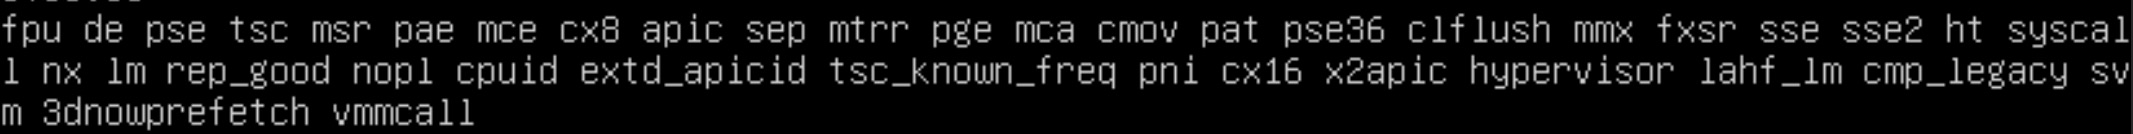
\includegraphics[width=1\textwidth]
    {assets/pics/lscpu_original.jpeg}
    \caption{Flag default KVM}
    \label{fig:lscpu_original}
\end{figure}

Terlihat pada gambar \ref{fig:lscpu_original} sama dengan Gambar \ref{fig:flag_kvm_host} di text yang ditebalkan. Dalam penelitian ini, flag yang akan diuji adalah \texttt{ssse3, sse4.1, sse4.2, sse4a, dan aes}. Semua flag SSE akan digunakan untuk percobaan kompresi video, sementara sse4.2 akan digunakan untuk validasi integritas data dengan CRC32, dan flag AES akan digunakan untuk enkripsi menggunakan AES. Harapannya, konfigurasi ini akan memberikan peningkatan kinerja yang signifikan dibandingkan dengan konfigurasi default dari KVM.

Untuk melakukan konfigurasi flag pada Hypervisor KVM, langkah pertama yang harus dilakukan adalah melihat daftar lengkap virtual machine yang sedang berjalan di sistem. Hal ini dapat dilakukan dengan menggunakan perintah:

\begin{listing}[H]
    \begin{minted}{bash}
    $ sudo virsh list
    \end{minted}
\end{listing}

Keluaran dari perintah ini adalah:
\begin{figure}
    \centering
    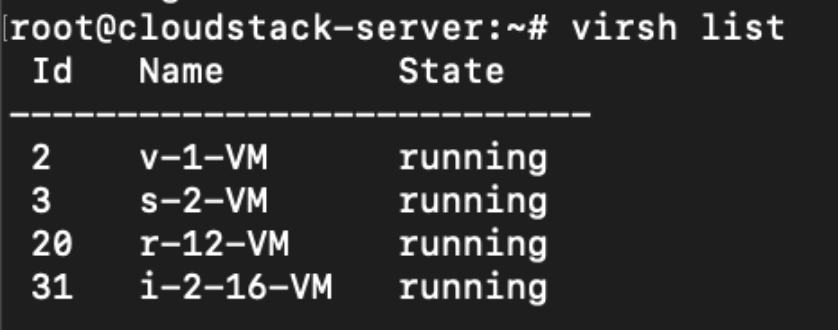
\includegraphics[width=0.5\textwidth]
    {assets/pics/virsh_list.png}
    \caption{Keluaran perintah \texttt{virsh list}}
    \label{fig:virsh_list}
\end{figure}

Pada Gambar \ref{fig:virsh_list} terlihat daftar virtual machine yang sedang berjalan di sistem. Dari daftar ini, virtual machine yang akan dikonfigurasikan adalah \texttt{i-2-16-VM}. Setelah mendapatkan nama virtual machine yang akan di-konfigurasi (\texttt{i-2-16-VM}), gunakan perintah \texttt{virsh edit i-2-16-VM} untuk melihat konfigurasi virtual machine tersebut.

\begin{figure}
    \centering
    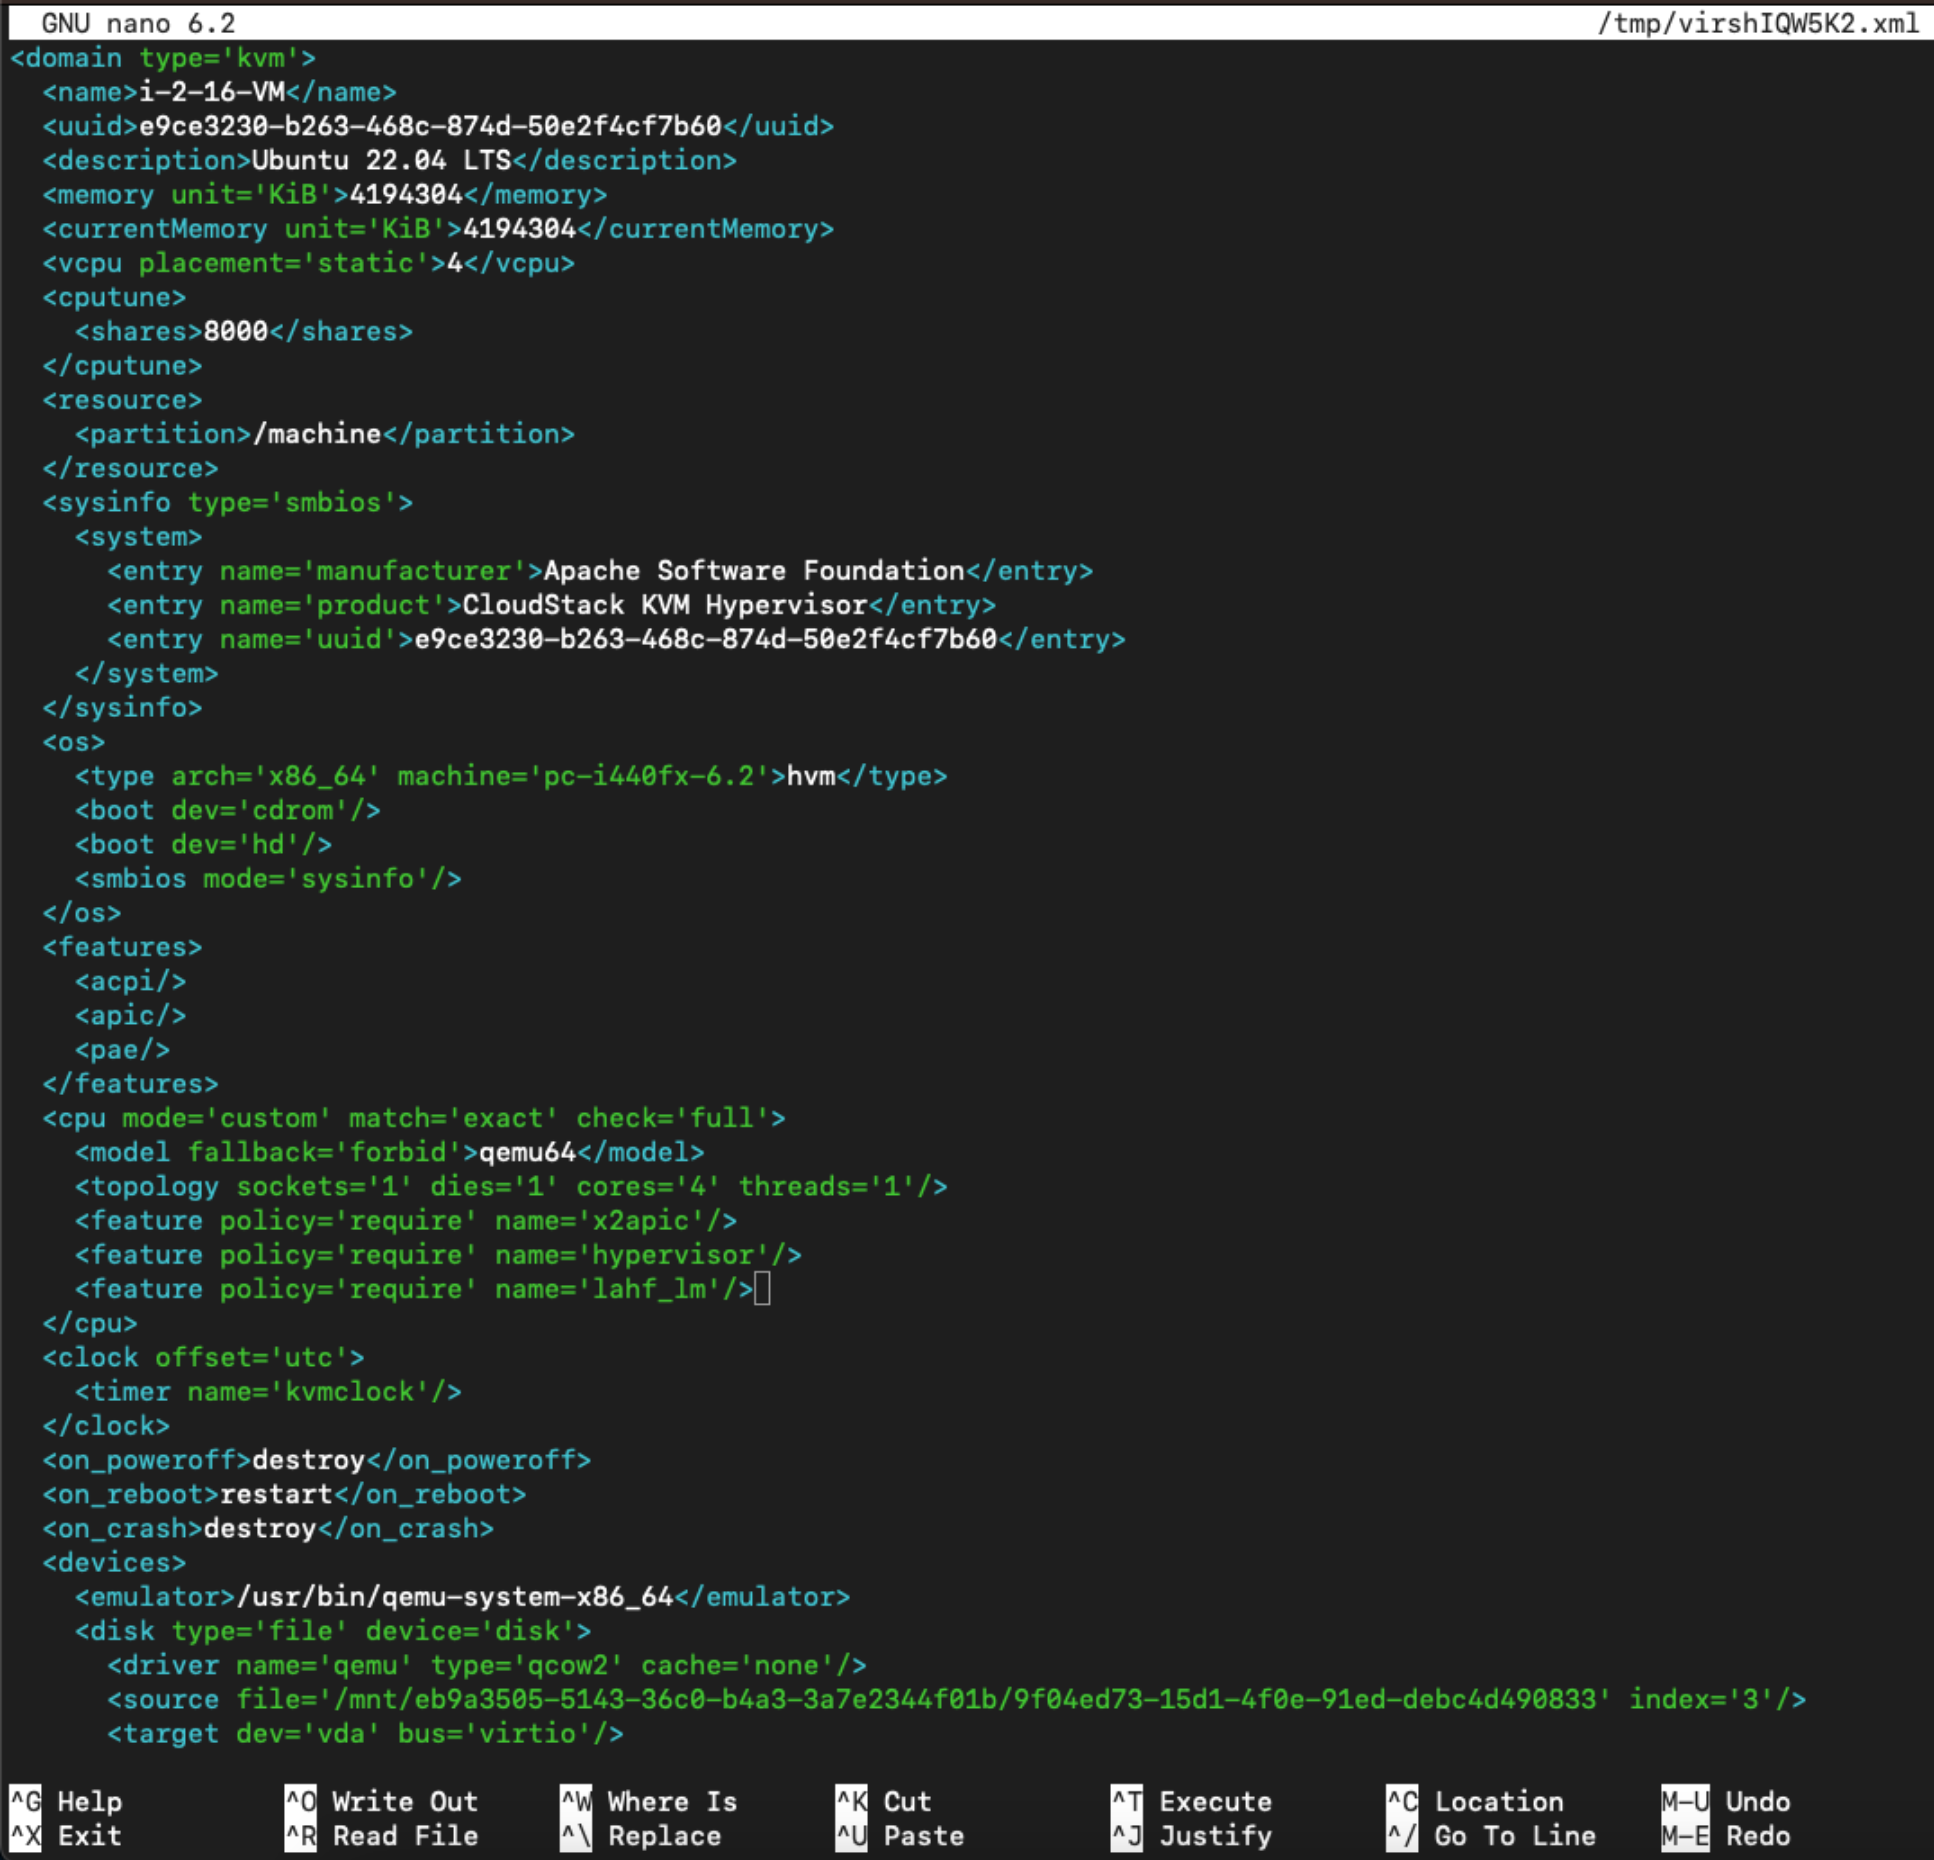
\includegraphics[width=0.9\textwidth]
    {assets/pics/virsh_edit1.png}
    \caption{Perintah \texttt{virsh edit i-2-16-VM} untuk melihat konfigurasi virtual machine \texttt{i-2-16-VM}}
    \label{fig:virsh_edit1}
\end{figure}

Pada gambar \ref{fig:virsh_edit1} terlihat konfigurasi virtual machine \texttt{i-2-16-VM}. Dari konfigurasi ini kita akan fokus pada bagian:

\begin{listing}[H]
    \begin{minted}{xml}
        ...

        <cpu mode='custom' match='exact' check='full'>
            <model fallback='forbid'>qemu64</model>
            <topology sockets='1' dies='1' cores='4' threads='1'/>
            <feature policy='require' name='x2apic'/>
            <feature policy='require' name='hypervisor'/> 
            <feature policy='require' name='lahf_1m'/>
        </cpu>
        
        ...
    \end{minted}
    \caption{Konfigurasi flag default}
    \label{code:default_kvm_xml}
\end{listing}

Kode \ref{code:default_kvm_xml} menampilkan konfigurasi flag default dari hypervisor KVM. Langkah berikutnya adalah menambahkan flag instruksi yang tidak termasuk dalam konfigurasi KVM default. Untuk melakukan ini, dilakukan duplikasi konfigurasi tersebut ke dalam sebuah file baru, seperti dalam penelitian ini yang akan disimpan di file \texttt{tuned\_kvm.xml}. Setelah disimpan di file \texttt{tuned\_kvm.xml}, selanjutnya dilakukan penambahan fitur yang diinginkan.

\begin{listing}[H]
    \begin{minted}{xml}
        ...

        <cpu mode='custom' match='exact' check='full'>
            <model fallback='forbid'>qemu64</model>
            <topology sockets='1' dies='1' cores='4' threads='1'/>
            <feature policy='require' name='x2apic'/>
            <feature policy='require' name='hypervisor'/> 
            <feature policy='require' name='lahf_1m'/>
            <feature policy='require' name='ssse3'/>
        </cpu>
        
        ...
    \end{minted}
    \caption{Konfigurasi flag ssse3}
    \label{code:ssse3_kvm_xml}
\end{listing}

Pada kode \ref{code:ssse3_kvm_xml}, fitur \texttt{ssse3} ditambahkan dengan menambahkan baris \texttt{<feature policy='require' name='ssse3'/>} pada kode tersebut. Setelah mengubah file \texttt{tuned\_kvm.xml}, \saya\ menyimpan perubahan pada file tersebut. Selanjutnya, mematikan mesin virtual dengan menggunakan perintah \texttt{destroy}:

\begin{listing}[H]
    \begin{minted}{bash}
    $ sudo virsh destroy i-2-16-VM
    \end{minted}
\end{listing}

Setelah virtual machine dimatikan, langkah selanjutnya adalah membuat virtual machine baru berdasarkan konfigurasi yang telah diubah sebelumnya. Hal ini dapat dilakukan dengan menggunakan perintah:

\begin{listing}[H]
    \begin{minted}{bash}
    $ sudo  virsh create tuned_kvm.xml
    \end{minted}
\end{listing}

Dengan perintah ini maka \vm\ \texttt{i-2-16-VM} akan dibuat menggunakan konfigurasi \texttt{tuned\_kvm.xml}. Kita dapat melihat perubahan pada \vm\ \texttt{i-2-16-VM} dengan menggunakan perintah \texttt{lscpu} pada console virtual machine.

\begin{figure}
    \centering
    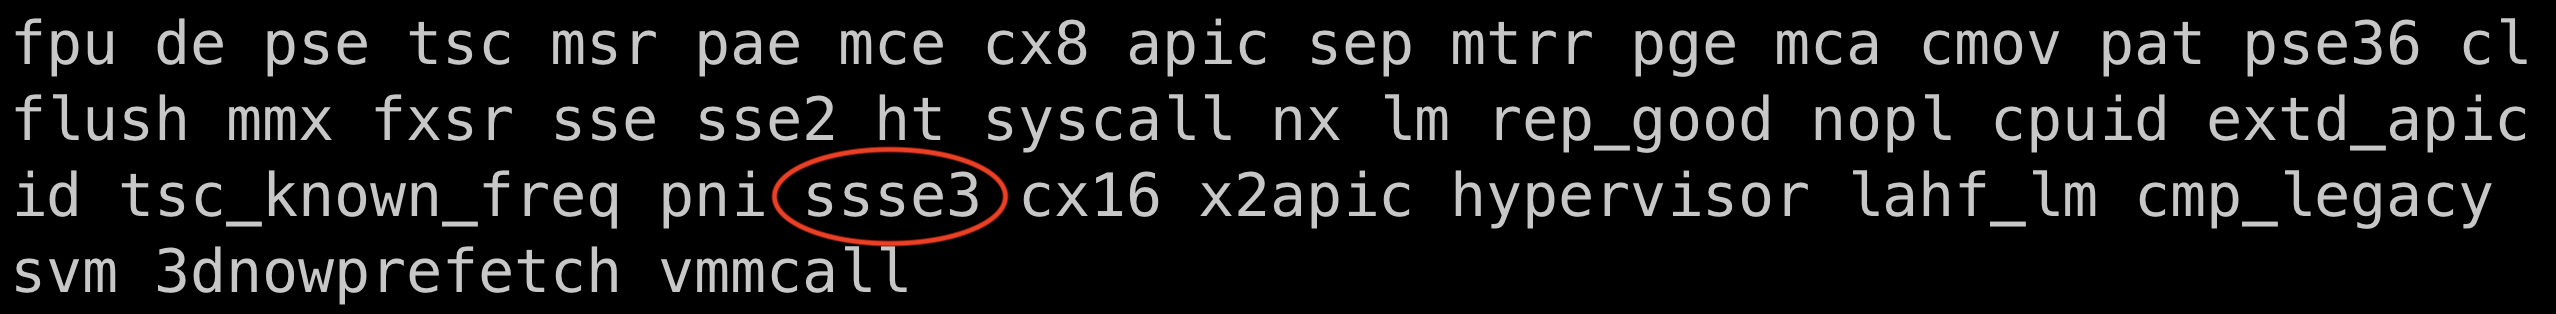
\includegraphics[width=1\textwidth]
    {assets/pics/lscpu_ssse3.jpeg}
    \caption{Flag tuned dengan ssse3}
    \label{fig:lscpu_ssse3}
\end{figure}

Dengan ini menandakan bahwa flag \texttt{ssse3} pada \vm\ \texttt{i-2-16-VM} sudah diaktifkan dan Hypervisor KVM sudah berhasil dikonfigurasikan.

%-----------------------------------------------------------------------------%
\subsection{Konfigurasi Hypervisor KVM untuk Kompresi Video}
%-----------------------------------------------------------------------------%
Pengujian kompresi video akan menggunakan konfigurasi seperti terlihat pada kode \ref{code:tuned_kompresi_video} yaitu dengan menggunakan flag ssse3, sse4.1, sse4.2, dan sse4a. Pemilihan flag-flag ini didasarkan pada instruksi SIMD (Single Instruction, Multiple Data) yang digunakan untuk operasi vektor pada data. Instruksi SIMD memungkinkan prosesor melakukan operasi secara bersamaan pada beberapa elemen data, sehingga mempercepat proses kompresi video dengan memanfaatkan kemampuan tersebut.

\begin{listing}[H]
    \begin{minted}{xml}
        ...

        <cpu mode='custom' match='exact' check='full'>
            <model fallback='forbid'>qemu64</model>
            <topology sockets='1' dies='1' cores='4' threads='1'/>
            <feature policy='require' name='x2apic'/>
            <feature policy='require' name='hypervisor'/> 
            <feature policy='require' name='lahf_1m'/>
            <feature policy='require' name='ssse3'/>
            <feature policy='require' name='sse4.1'/>
            <feature policy='require' name='sse4.2'/>
            <feature policy='require' name='sse4a'/>
        </cpu>
        
        ...
    \end{minted}
    \caption{Konfigurasi Hypervisor KVM untuk Kompresi Video}
    \label{code:tuned_kompresi_video}
\end{listing}

%-----------------------------------------------------------------------------%
\subsection{Konfigurasi Hypervisor KVM untuk Validasi Integritas Data}
%-----------------------------------------------------------------------------%
Untuk melakukan pengujian dengan validasi integritas data akan digunakan konfigurasi seperti pada kode \ref{code:tuned_validasi_integritas_file}. Flag yang akan digunakan adalah sse4.2. Flag ini dipilih dikarenakan salah satu kemampuan yang dimiliki oleh flag ini adalah mendukung instruksi CRC32 yang akan digunakan untuk validasi integritas data.

\begin{listing}[H]
    \begin{minted}{xml}
        ...

        <cpu mode='custom' match='exact' check='full'>
            <model fallback='forbid'>qemu64</model>
            <topology sockets='1' dies='1' cores='4' threads='1'/>
            <feature policy='require' name='x2apic'/>
            <feature policy='require' name='hypervisor'/> 
            <feature policy='require' name='lahf_1m'/>
            <feature policy='require' name='sse4.2'/>
        </cpu>
        
        ...
    \end{minted}
    \caption{Konfigurasi Hypervisor KVM untuk Validasi Integritas Data}
    \label{code:tuned_validasi_integritas_file}
\end{listing}

%-----------------------------------------------------------------------------%
\subsection{Konfigurasi Hypervisor KVM untuk Enkripsi dan Dekripsi AES}
%-----------------------------------------------------------------------------%
Untuk melakukan pengujian dengan enkripsi AES akan digunakan konfigurasi seperti pada kode \ref{code:tuned_enkripsi_aes}. Flag yang akan digunakan adalah aes. Flag ini dipilih dikarenakan salah satu kemampuan yang dimiliki oleh flag ini adalah mendukung instruksi AES yang akan digunakan untuk enkripsi AES.

\begin{listing}[H]
    \begin{minted}{xml}
        ...

        <cpu mode='custom' match='exact' check='full'>
            <model fallback='forbid'>qemu64</model>
            <topology sockets='1' dies='1' cores='4' threads='1'/>
            <feature policy='require' name='x2apic'/>
            <feature policy='require' name='hypervisor'/> 
            <feature policy='require' name='lahf_1m'/>
            <feature policy='require' name='aes'/>
        </cpu>
        
        ...
    \end{minted}
    \caption{Konfigurasi Hypervisor KVM untuk Enkripsi AES}
    \label{code:tuned_enkripsi_aes}
\end{listing}

%-----------------------------------------------------------------------------%
\section{Skenario Pengujian Konfigurasi}
%-----------------------------------------------------------------------------%
Pada bagian ini akan dijelaskan skenario pengujian yang akan dilakukan untuk mengukur dampak konfigurasi yang dilakukan pada Hypervisor KVM terhadap kinerja virtual machine. Pengujian akan dilakukan dengan menggunakan tiga skenario yang berbeda, yaitu kompresi video, validasi integritas data, dan enkripsi dan dekripsi AES. Setiap skenario akan dijalankan pada virtual machine yang telah dikonfigurasikan dengan konfigurasi yang sesuai.

%-----------------------------------------------------------------------------%
\subsection{Skenario Pengujian Kompresi Video}
%-----------------------------------------------------------------------------%
\begin{figure}
    \centering
    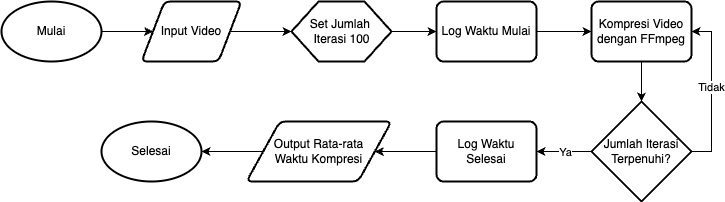
\includegraphics[width=1\textwidth]
    {assets/pics/code-flowchart/flowchart_kompresi_video.png}
    \caption{Flowchat Kode Pengujian Kompresi Video}
    \label{fig:flowchart_kompresi_video}
\end{figure}

Pada pengujian kompresi video akan dilakukan dengan menggunakan perangkat lunak ffmpeg untuk melakukan kompresi video. Flow untuk melakukan pengujian dengan kompresi video dapat terlihat di gambar \ref{fig:flowchart_kompresi_video}. Pengujian ini akan mengukur waktu yang diperlukan untuk melakukan kompresi video dengan menggunakan konfigurasi yang telah dilakukan pada Hypervisor KVM. Pengujian ini akan dilakukan dengan menggunakan video yang berjudul \texttt{Times Square Day Wide} yang memiliki durasi 10 detik dan resolusi 4k. Video ini akan dikompresi menggunakan codec h265 dengan preset medium. Pengujian akan dijalankan sebanyak 100 kali per konfigurasi dan diukur waktu yang diperlukan untuk menyelesaikan proses kompresi video. Script bash lengkap yang digunakan untuk melakukan pengujian kompresi video dapat dilihat di \textbf{kode \ref{code:kode_pengujian_kompresi_video}} pada lampiran.

%-----------------------------------------------------------------------------%
\subsection{Skenario Pengujian Validasi Integritas Data}
%-----------------------------------------------------------------------------%
\begin{figure}
    \centering
    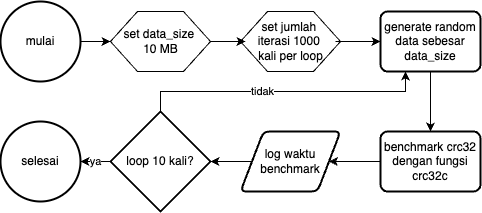
\includegraphics[width=1\textwidth]
    {assets/pics/code-flowchart/flowchart_crc32.png}
    \caption{Flowchat Kode Pengujian Validasi Integritas Data}
    \label{fig:flowchart_crc32}
\end{figure}

Pada pengujian validasi integritas data akan dilakukan dengan menggunakan library crc32c dari python untuk melakukan validasi pada sebuah data. Flow untuk melakukan pengujian validasi integritas data dapat dilihat pada gambar \ref{fig:flowchart_crc32}. Pengujian ini akan mengukur waktu yang diperlukan untuk melakukan perhitungan CRC32 pada data bytearray yang berukuran 10 MB. Pengujian ini akan dijalankan sebanyak 100 kali per konfigurasi kemudian diukur waktu yang diperlukan untuk menyelesaikan proses perhitungan CRC32. Kode python lengkap yang digunakan untuk melakukan pengujian validasi integritas data dapat dilihat di \textbf{kode \ref{code:kode_pengujian_validasi_integritas_data}} pada lampirn.

%-----------------------------------------------------------------------------%
\subsection{Skenario Pengujian Enkripsi dan Dekripsi AES}
%-----------------------------------------------------------------------------%
\begin{figure}
    \centering
    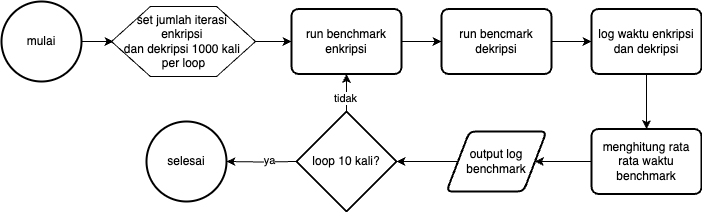
\includegraphics[width=1\textwidth]
    {assets/pics/code-flowchart/flowchart_aes.png}
    \caption{Flowchat Kode Pengujian Enkripsi dan Dekripsi AES}
    \label{fig:flowchart_aes}
\end{figure}

Pada pengujian enkripsi dan dekripsi AES akan dilakukan dengan menggunakan library cryptography dari python untuk melakukan enkripsi AES. Flow untuk melakukan pengujian dengan enkripsi dan dekripsi AES dapat dilihat pada gambar \ref{fig:flowchart_aes} Pengujian ini akan mengukur waktu yang diperlukan untuk melakukan enkripsi AES pada data teks yang dapat dilihat pada Gambar \ref{fig:aesPlaintextData}. Pengujian ini akan dijalankan sebanyak 100 kali per konfigurasi dan diukur waktu yang diperlukan untuk menyelesaikan proses enkripsi dan dekripsi AES. Kode python yang digunakan untuk melakukan pengujian enkripsi AES dapat dilihat di \textbf{kode \ref{code:pengujian_enkripsi_aes}} pada lampiran.

%-----------------------------------------------------------------------------%
\section{Skenario Analisis}
%-----------------------------------------------------------------------------%
Analisis akan dilakukan dengan melakukan perhitungan menggunakan formula \texttt{speedup}. Diasumsikan bahwa T(1) adalah waktu eksekusi Test dengan konfigurasi default, dan T(p) adalah waktu eksekusi Test dengan konfigurasi yang telah dikonfigurasikan \cite{beuwolfCetin}.

Formula \texttt{speedup} dinyatakan sebagai berikut:

\begin{equation}
    S(p) = \frac{T(1)}{T(p)}
    \label{eq:formula}
\end{equation}

Berdasarkan rumus \ref{eq:formula}, jika nilai S(p) semakin besar, maka konfigurasi yang dikonfigurasikan semakin bagus. Hal ini menandakan bahwa konfigurasi Hypervisor dapat mempercepat proses yang dilakukan. Sebaliknya, jika S(p) semakin kecil, maka konfigurasi yang dikonfigurasikan semakin lambat. Jika nilai S(p) sama, maka efek dari konfigurasi yang dikonfigurasikan sama dengan konfigurasi default.

Dalam analisis pengujian dengan kompresi video, \saya\ akan membandingkan waktu eksekusi antara konfigurasi Hypervisor yang tidak dikonfigurasikan (default) dan konfigurasi yang telah dikonfigurasikan. Perbandingan ini akan dilakukan dengan menggunakan formula \texttt{speedup}. Konfigurasi yang optimal adalah konfigurasi yang memiliki nilai \texttt{speedup} tertinggi, yang menunjukkan peningkatan kinerja yang signifikan dalam proses kompresi video.

Untuk analisis pengujian validasi integritas data, \saya\ akan menggunakan pendekatan yang serupa dengan analisis kompresi video. Akan dibandingkan waktu eksekusi antara konfigurasi Hypervisor yang tidak dikonfigurasikan (default) dan konfigurasi yang telah dikonfigurasikan menggunakan formula \texttt{speedup}. Nilai S(p) yang lebih besar menunjukkan bahwa konfigurasi yang dikonfigurasikan lebih efisien dalam memverifikasi integritas data dibandingkan dengan konfigurasi default.

Dalam analisis pengujian enkripsi AES, \saya\ akan menggunakan metode yang sama seperti analisis sebelumnya, yaitu dengan membandingkan waktu eksekusi antara konfigurasi Hypervisor yang tidak dikonfigurasikan (default) dan konfigurasi yang telah dikonfigurasikan menggunakan formula \texttt{speedup}. Nilai S(p) yang lebih besar menunjukkan bahwa konfigurasi yang dikonfigurasikan lebih efisien dalam melakukan enkripsi AES dibandingkan dengan konfigurasi default.

Dengan menganalisis nilai \texttt{speedup}, penulis dapat mengevaluasi dan membandingkan kinerja berbagai konfigurasi Hypervisor dalam melakukan tugas-tugas seperti kompresi video, validasi integritas data, dan enkripsi AES. Konfigurasi dengan nilai \texttt{speedup} tertinggi akan menjadi pilihan yang optimal untuk meningkatkan kinerja dan efisiensi dalam setiap tugas yang diuji.